\setchaptertoc
\chapter{Introduction}\label{chp:introduction}
\csummary{What is the problem solved by this thesis?\csumnext What are our research questions?\csumnext What are our contributions?}

\section{Motivation}

Sample cite~\cite{DBLP:conf/msr/SihlerPSTDD24}

\begin{minted}{R}
x <- list(i='hey', j='there')
for(i in x) {
   print(paste("x$i", x$i))
}
print(x)
\end{minted}


To interpret the program above, we take \bR{x <- 2} to the set of \gls{not:N}, \gls{not:Z}, and \gls{not:R} because they describe funny numbers that we can use to index what we call an \gls{ast} (if you want the long form use \texttt{\textbackslash glsac}: \glsac{ast}). Now we can use a \gls{cpo} or verify the \gls{def:behavioral-equivalence} with \glspl{formal:external-factor} when interpreting the code as a \Gls{formal:model} (see \gls{def:behavioral-equivalence}, sometimes called \gls{def:behavioral-equivalence}[foo bar]).
\gls{not:N} will not be repeated on this page!

Using the \texttt{\textbackslash glssym} macro defined in the preamble you can even color symbol uses such as \glssym{not:N} automatically if this is to your liking:
\begin{align}
   \glssym{not:N} &= \{1, 2, \ldots\} \\
   \glssym{not:Z} &= \glssym{not:N} \cup \{0\} \cup \{-1, -2, \ldots\} \\
   \glssym{not:R} &= \textit{Set of real numbers} \\
   \glssym{not:C} &= \textit{Set of complex numbers} \\
   \glssym{not:N} &\subset \glssym{not:Z} \subset \glssym{not:R} % \subset \glssym{not:C}
\end{align}

However, as you may see, \glssym{not:C} is not shown in the sidebar even though it appears first within the math mode. The reason(s) for this are manifold but in short we avoided this as math mode may be rendered multiple times. 
You can use \texttt{\textbackslash showsymbols} to propose a list of symbols to show before the math environment (using \texttt{\textbackslash showsymbols*} these will be forced as showcased below):
\begin{align}
   \showsymbols*{not:N,not:Z,not:R,not:C}
   \glssym{not:N} &= \{1, 2, \ldots\} \\
   \glssym{not:Z} &= \glssym{not:N} \cup \{0\} \cup \{-1, -2, \ldots\} \\
   \glssym{not:R} &= \textit{Set of real numbers} \\
   \glssym{not:C} &= \textit{Set of complex numbers} \\
   \glssym{not:N} &\subset \glssym{not:Z} \subset \glssym{not:R} % \subset \glssym{not:C}
\end{align}

\clearpage
\begin{figure}
   \begin{subfigure}[c]{0.33\linewidth}
      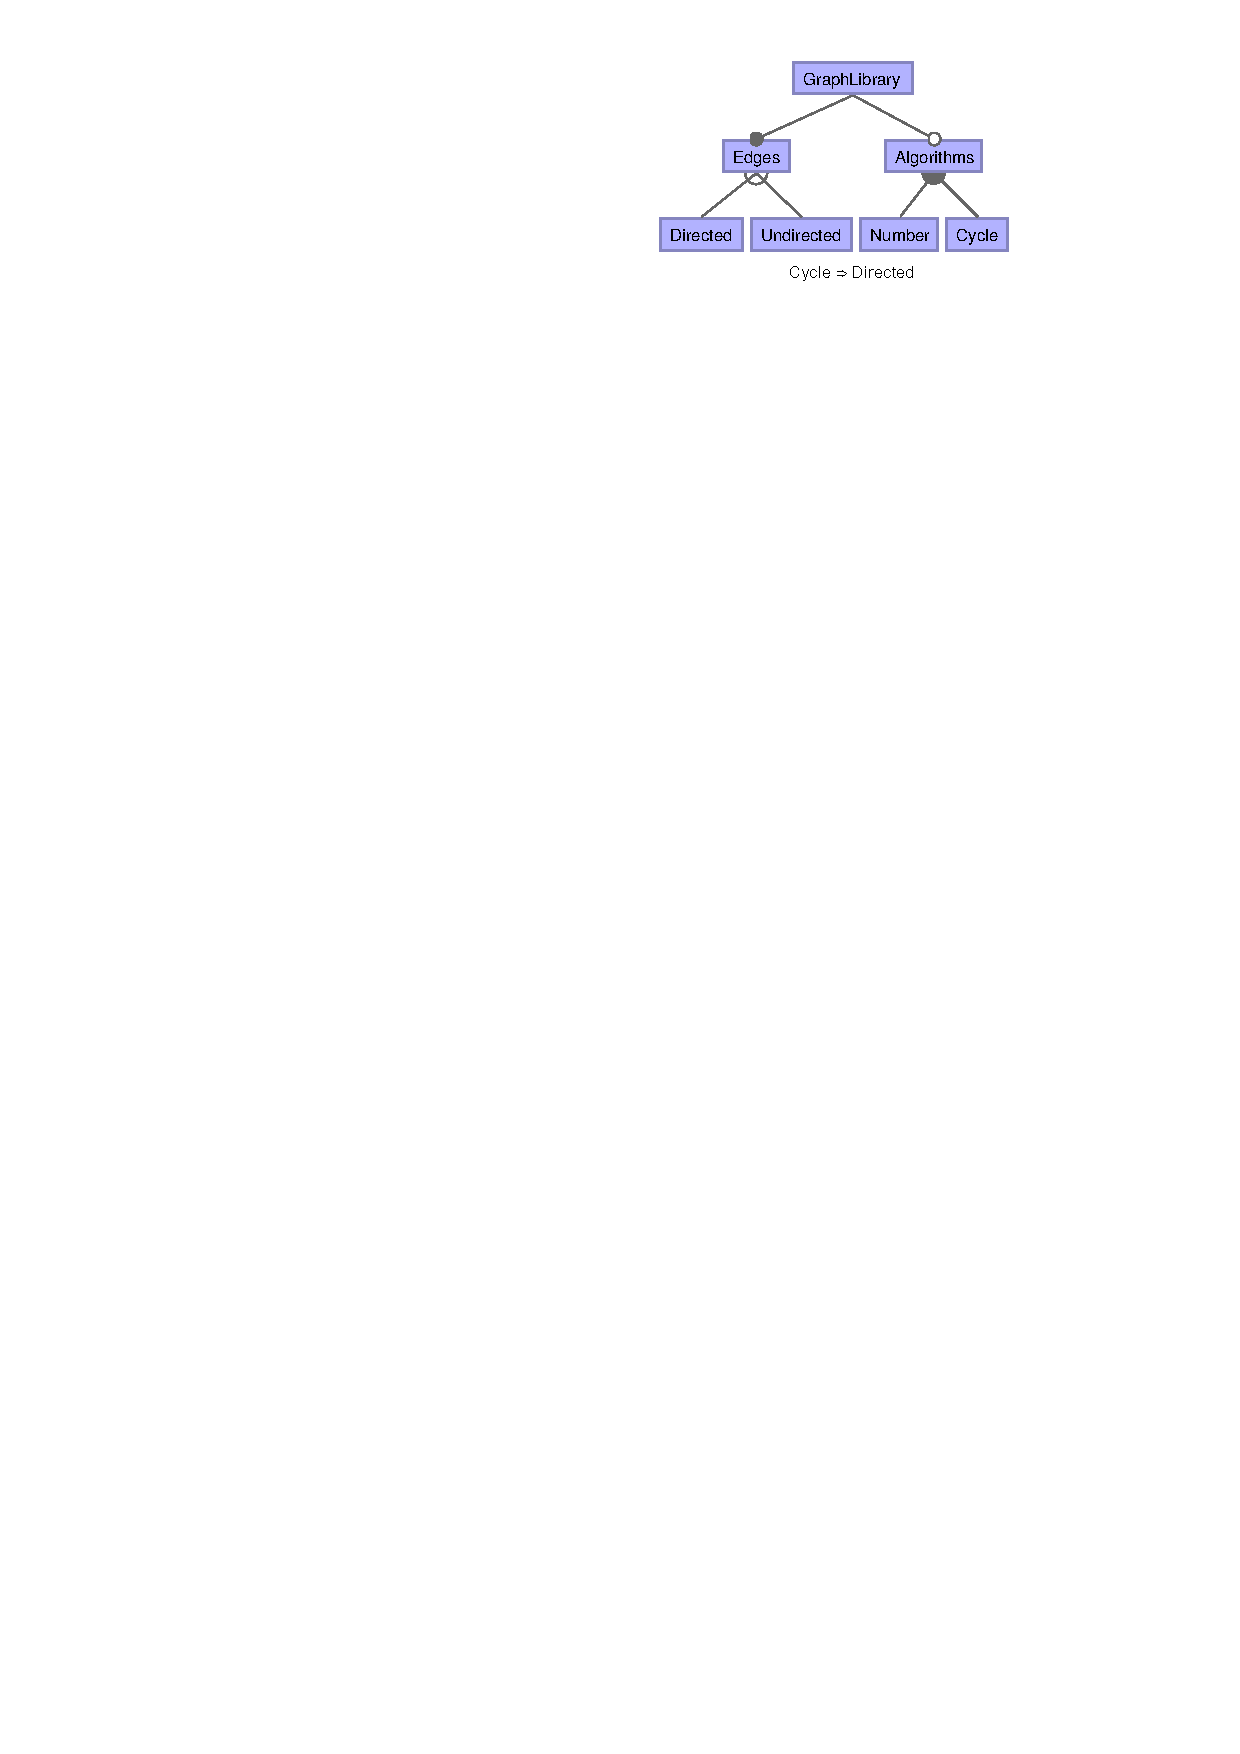
\includegraphics[width=\linewidth]{img/example.pdf}
      \caption{First subfigure.}
      \label{fig:first}
  \end{subfigure}\hfill
  \begin{subfigure}[c]{0.33\linewidth}
      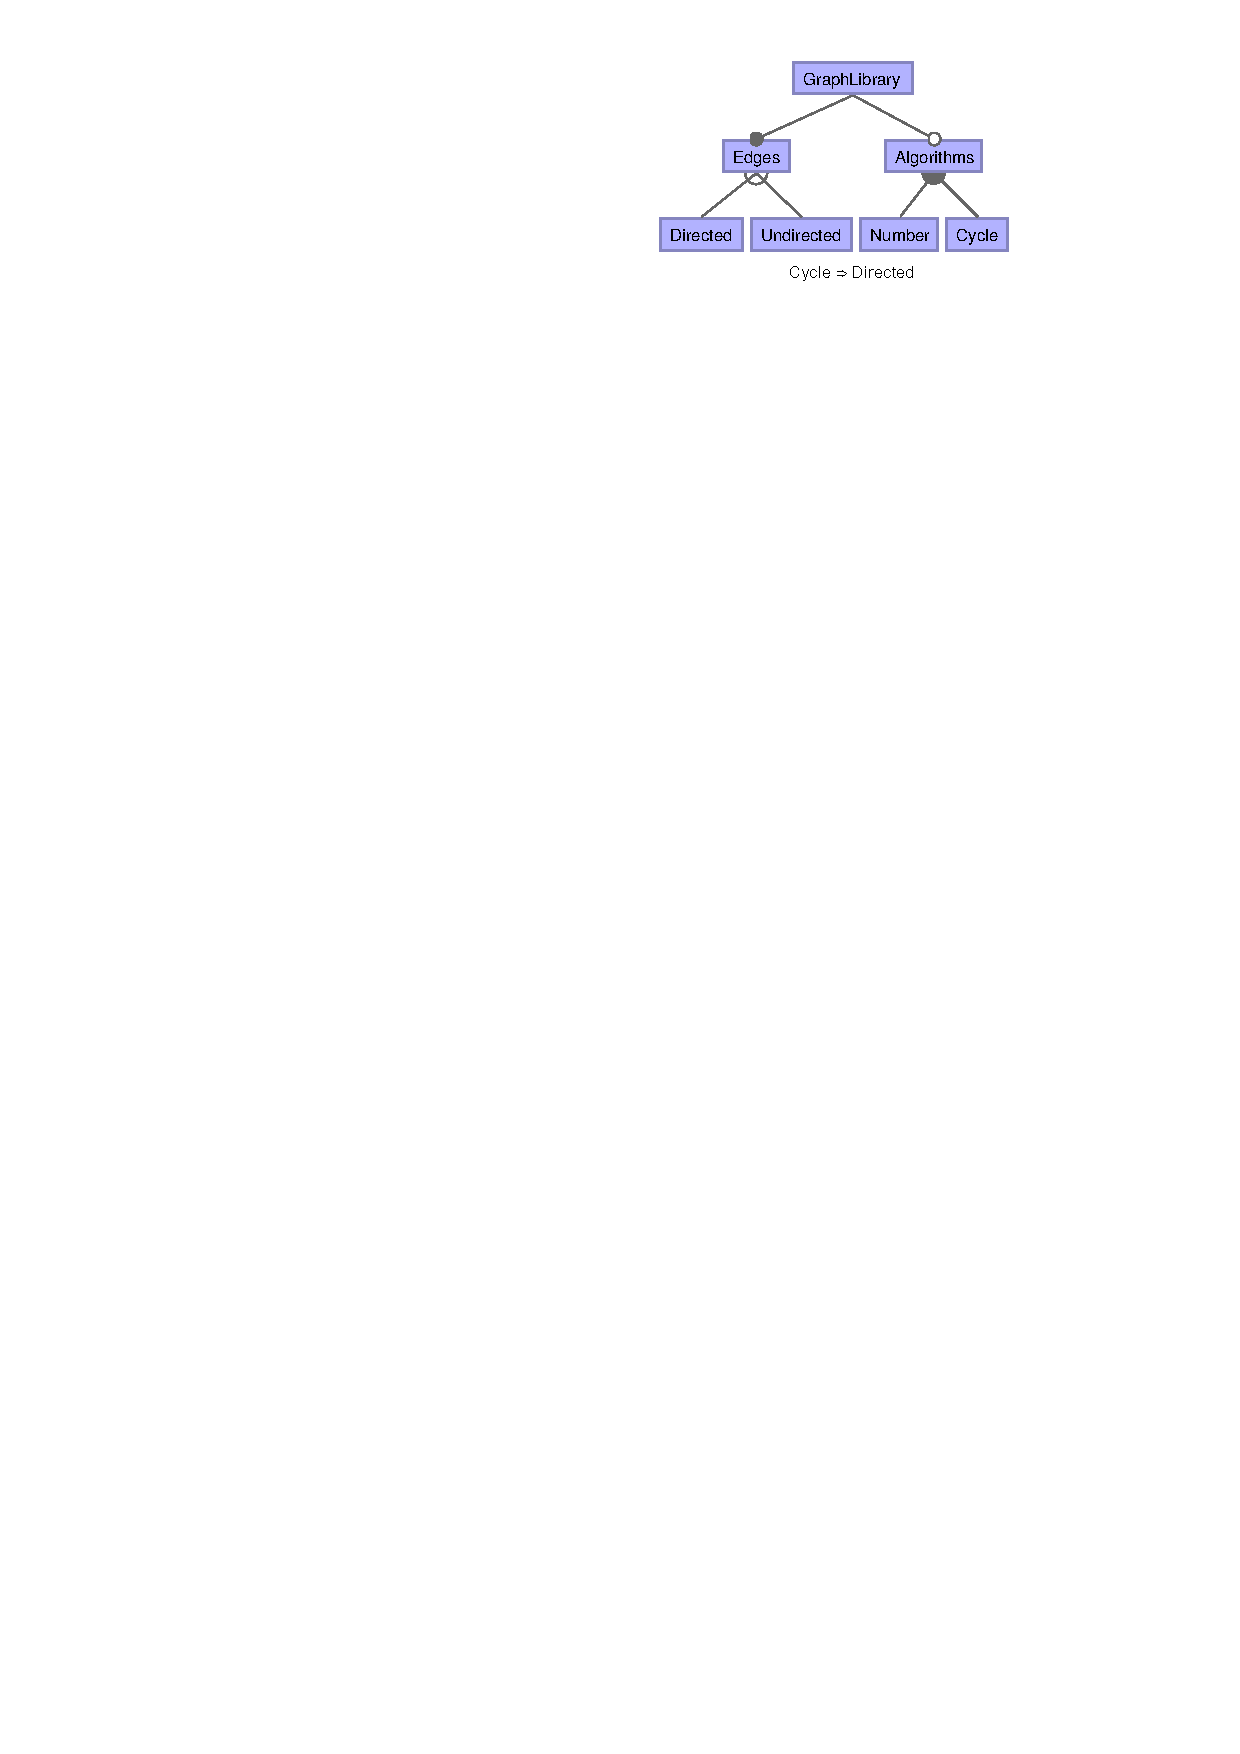
\includegraphics[width=\linewidth]{img/example.pdf}
      \caption{Second subfigure.}
   \end{subfigure}
   \caption[Main]{Main caption.}
   \label{fig:main}
\end{figure}

A viable way to group different figures is the \textit{subfigures} command, a short example can be seen at \cref{fig:main}.
This is \cref{fig:main} with the name \nameref{fig:main}.\footurl{www.google.com}{2024-12-24}
See ulm university\foothref{https://web.archive.org/web/20241221140233/https://www.uni-ulm.de/}{https://www.uni-ulm.de/}{2024-12-21} for more information.

\begin{table}
   \caption{A simple table}
   \begin{tabular}{cc}
      \toprule
      A & B \\
      \midrule
      1 & 2 \\
      3 & 4 \\
      \bottomrule
   \end{tabular}
   \label{tab:simple}
\end{table}

\section{Problem Statement}

\begin{pseudo}[tbp]
	\caption{Algo Good}
	\label{fun:good-algo}
	\begin{algorithm}[H]
		\PreCode
		\Input{x :: String}
      \Output{y :: String}
		\Output{z :: String}
		
		\StartCode
		\lIf{x \KwIs "hello"}{
         \label{alg:important-line}\Return{"world"}
      }
      \While{true}{
         \If{y \KwIs "world"}{
            \Return{"hello"}
         }
      }
      \Return{"goodbye"}
	\end{algorithm}
\end{pseudo}

In the \nameref{fun:good-algo} algorithm \cref{fun:good-algo}, an important line is \AlgoLineRef{alg:important-line}.

\section{Contributions}

\section{Overview}